\chapter{Implementierung}

\anno{max. 5 Seiten} %Ref hat 12

% Highlight 1 der Implementierung

Als Grundlage für die Implementierung der Firewall-Funktionalität wurde mit der Software \emph{WebCastellum} eine etwas ältere Implementierung eines Servlet-Filters gewählt.

\section{Vorarbeiten}

\begin{picture}[h]
  \centering
  \begin{gnuplot}[scale=.7]
    set datafile separator ','
    set xdata time
    set timefmt "%Y-%m"
    set xrange ["2009-01":"2022-04"]
    set format x "%b %y"
    set key autotitle columnhead
    plot '04_Implementierung/downloads.csv' using 1:2 with lines
  \end{gnuplot}
  \caption{Downloads Statistics WebCastellum 1.8.3 binary}
  \label{fig:downloadwc}
\end{picture}
  
\subsection{Review Quellcode und IT-Sicherheit}
\subsection{Unit-Tests etc.}
\subsection{Fehlerbereinigung}

% Highlight 2 der Implementierung
\section{Zentralisierung}
\begin{figure}[ht]
    \centering
    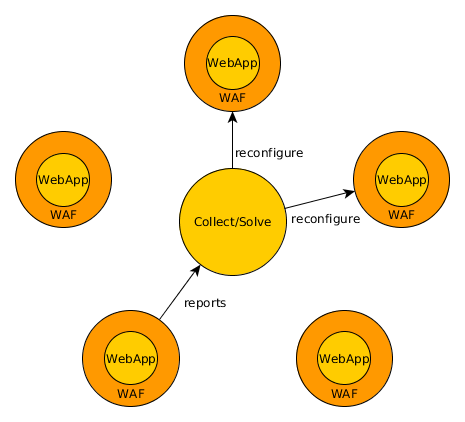
\includegraphics[width=8cm]{central.png}
    \caption{Arbeit der WAFs im Verbund}
    \label{fig:my_verbund}
\end{figure}

\begin{figure}[bht]
  \begin{center}
    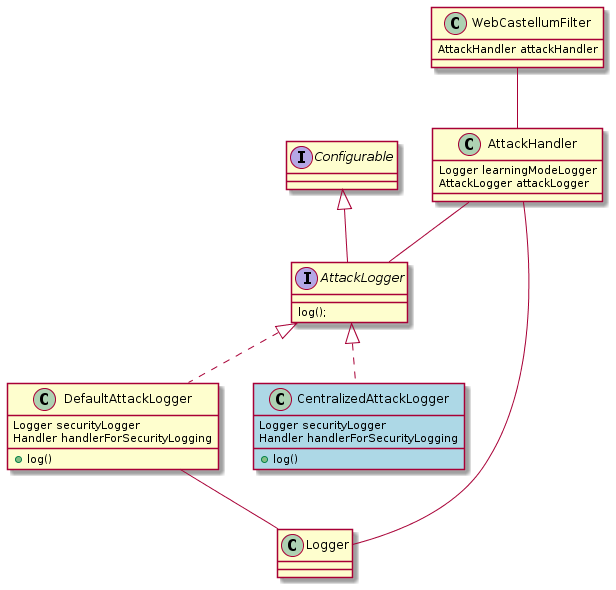
\includegraphics[width=12cm]{classp}
    \caption{Implementierung Nachrichtenversand}
    \label{fig.impversand}
  \end{center}
\end{figure}

\begin{figure}[h]
  \begin{center}
    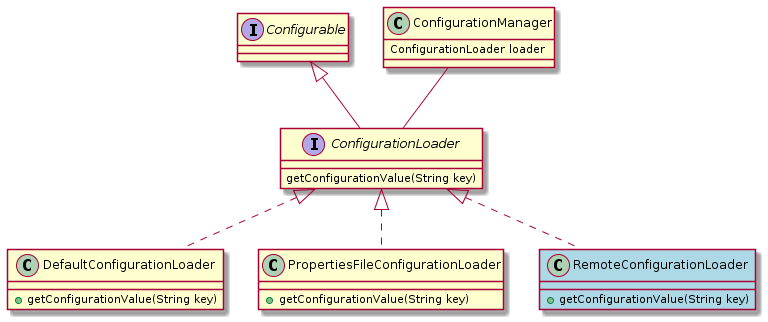
\includegraphics[width=14cm]{configclasses}
    \caption{Implementierung Konfiguration}
    \label{fig.impkonfig}
  \end{center}
\end{figure}



\section{ML-Fähigkeit}

\begin{figure}[h]
    \centering
    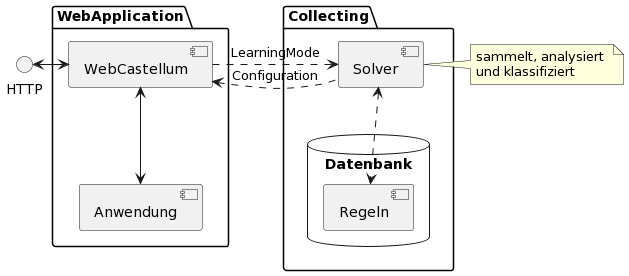
\includegraphics[width=9cm]{webcastellumcentral.png}
    \caption{Komponentendiagramm für zentrale Klassifizierung}
    \label{fig:my_future}
\end{figure}


% Highlight des Deployments beim Kunden

% Zusammenfassung: ca. 0,5 Seiten
\section{Zusammenfassung}



